\documentclass[11pt,a4paper]{article}

\usepackage[utf8]{inputenc}
\usepackage[T1]{fontenc}
\usepackage{lmodern}
\usepackage{microtype}
\usepackage[margin=2.5cm]{geometry}
\usepackage{amsmath,amssymb,amsthm}
\usepackage{mathtools}
\usepackage{booktabs}
\usepackage{array}
\usepackage{enumitem}
\usepackage{hyperref}
\usepackage{xcolor}
\usepackage{tcolorbox}
\usepackage{fancyhdr}
\usepackage{graphicx}

\hypersetup{colorlinks=true, linkcolor=blue!50!black,
  citecolor=blue!50!black, urlcolor=blue!50!black}

\pagestyle{fancy}
\fancyhf{}
\fancyhead[L]{\small Critical-line pull-back probe on $V_{600}$}
\fancyhead[R]{\small Pre-peer-review preprint}
\fancyfoot[C]{\thepage}

\newtheorem{finding}{Finding}

\newcommand{\II}{\mathcal{I}}
\newcommand{\Vsix}{V_{600}}
\newcommand{\Vtf}{V_{24}}
\newcommand{\Cphi}{C_\varphi}
\newcommand{\NH}{N_H}
\newcommand{\Q}{\mathbb{Q}}
\newcommand{\Z}{\mathbb{Z}}
\newcommand{\R}{\mathbb{R}}
\newcommand{\C}{\mathbb{C}}
\newcommand{\N}{\mathbb{N}}
\newcommand{\Lsub}{L_{\mathrm{sub}}}

\newtcolorbox{findingbox}[1][]{
  colback=blue!2,
  colframe=blue!40!black,
  fonttitle=\bfseries,
  #1
}

\newtcolorbox{scopebox}[1][]{
  colback=gray!4,
  colframe=gray!50!black,
  fonttitle=\bfseries,
  title=Scope,
  #1
}

\title{\textbf{The Critical Line, Pulled Back to $V_{600}$}\\[0.4em]
\large Computational checks around the icosian L-function
factorisation, led by one exact negative Galois result; nothing here
states or implies progress on RH or $\mathrm{GRH}_{\chi_5}$}

\author{Lee Smart\\
\small Institute of Vibrational Field Dynamics\\
\small \texttt{contact@vibrationalfielddynamics.org}}

\date{2026-06-12 \quad (pre-peer-review preprint, v1.1.0-rc1 --- revised after adversarial review)}

\begin{document}
\maketitle

\begin{abstract}
\noindent
The Riemann critical line is straight only in the coordinate $s$ of
the complex plane. Under the Hilbert modular L-function identity
$L(\Theta_\II, s) = \zeta_K(s) \cdot \zeta_K(s-1) \cdot C_2(s)$ for
$K = \Q(\sqrt 5)$, with $\zeta_K(s) = \zeta(s) \cdot L(s, \chi_5)$,
the critical line of $\zeta(s)$ pulls back to a curve on the
icosian substrate. This paper reports computational checks at three
distinct grades --- a pipeline sanity check and two verified finite
computations (Findings 1--3), one exact negative result which is
the principal finding (Finding 4), and four exploratory follow-ons
stamped as such (Findings 5--8) --- from a multi-version probe
simulation that builds $\Vsix$ exactly,
constructs the substrate L-function analytically using
\texttt{mpmath}, evaluates it at the first ten Riemann zeros, and
verifies the Eichler--Brandt representation formula at finite
coordinate bound.

The findings are:
\begin{enumerate}[leftmargin=*]
  \item The substrate L-function vanishes at every one of the first
        ten Riemann zeros to numerical precision
        ($|L_{\mathrm{sub}}(1/2 + i \gamma_n)| < 2.2 \cdot 10^{-11}$ for
        $n = 1, \ldots, 10$). This is the empirical image of the
        critical line on the substrate.
  \item The Eichler--Brandt formula $r(p) = 8 (1 + p^2)$ for odd
        rational primes $p$ inert in $\Z[\varphi]$ is reproduced
        exactly at coordinate bound $K = 4$ for every inert prime
        tested ($p \in \{3, 7, 13, 17, 23\}$), together with the
        Jacobi-style anomaly $r(2) = 24$.
  \item A clean closed 10-vertex icosian rotation orbit can be
        exhibited as a discrete helix on $S^3$ --- a group-action
        demonstration; the relation to the continuous L-spiral is
        left open.
  \item Coordinate-Galois $\sigma$ \emph{does not preserve $\Vsix$
        as a set}: $96$ of the $120$ vertices map under
        $\varphi \mapsto 1 - \varphi$ to odd-permutation positions
        in the icosian ring, outside the even-permutation $\Vsix$.
        The ``$94 + 13 + 13$'' $\sigma$-pairing decomposition cited
        in the icosian-triad paper must reference a different
        involution $\tau$ on the operator algebra, not the direct
        coordinate-Galois action.
  \item (Follow-on to Finding 4, bookkeeping level.) Grouping the
        $\Cphi$ eigenvalues by Galois conjugacy of their values
        partitions multiplicities as $94 + 13 + 13 = 120$ exactly:
        five rational $A_1$ eigenvalues $\{12, 3, 0, -2, -3\}$
        (mults $1, 16, 25, 36, 16$) and two Galois-paired sets
        ($4{+}4$ and $9{+}9$). This identifies a natural
        \emph{candidate} for the involution $\tau$ at the level
        of spectral data; constructing $\tau$ as an involution on
        the vertex space or operator algebra is not done here.
        Separately, at each tabulated $\gamma_n$ the $\zeta$
        factor is at machine zero while $|L(1/2+i\gamma_n,
        \chi_5)|$ is order one --- a scalar attribution of each
        zero to the $\sigma$-fixed Dedekind factor; no projection
        of zeros into a $94$-dimensional space is computed.
  \item (Operator-level support for H-attr.) Four natural
        closure-flow dynamics on $\Vsix$ all drive the $26$-dim
        $\tau$-paired component to zero (or, when $\tau$-asymmetric
        noise is added, to a small equilibrium of order $\sim 5
        \cdot 10^{-3}$). The block structure of $\Cphi$ is
        verified to machine precision
        ($\|[\Cphi, P_+]\|_\infty < 2 \cdot 10^{-15}$;
        $\mathrm{tr}\,P_+ = 94$, $\mathrm{tr}\,P_- = 26$). The
        toy dynamics are consistent with H-attr; they do not
        establish it.
\end{enumerate}

We make no claim of settling the Riemann Hypothesis. We claim only
that the substrate image of $\zeta$'s critical line is exhibited
explicitly, the prime representation counts are confirmed at the
formula's quoted precision, and the open follow-on (identification
of the $\tau$-involution carrying the $94 + 13 + 13$ split) is
pinned down to a precise mathematical statement.
\end{abstract}

\bigskip

\noindent\textbf{Status.} Pre-peer-review open research preprint.
Not independently validated. No claim of RH / GRH settlement is
made anywhere.

\tableofcontents

\newpage

\section{Setting: where the critical line sits on $V_{600}$}
\label{sec:setting}

The icosian theta L-function on the maximal order $\II$ over
$K = \Q(\sqrt 5)$ satisfies the factorisation identity
\begin{equation}
\label{eq:factorisation}
  L(\Theta_\II, s) \;=\; \zeta_K(s)\,\zeta_K(s-1)\,C_2(s),
  \qquad
  C_2(s) \;=\; 1 - 2 \cdot 2^{-s} + 2^{2-2s},
\end{equation}
with Dedekind splitting
$\zeta_K(s) = \zeta(s) \cdot L(s, \chi_5)$ where $\chi_5$ is the
unique non-trivial quadratic Dirichlet character modulo $5$. This
identity is proved unconditionally in \cite{icosianTriad} and
verified numerically at multiple values of $s$ in the bundle's
reproduction suite (sim 13 of \cite{icosianTriad}).

Equation \eqref{eq:factorisation} provides the explicit map under
which the analytic critical line $\mathrm{Re}(s) = 1/2$, on which
$\zeta(s)$ has its non-trivial zeros, is identified with a curve
on the substrate. The curve is parametrised by
$\gamma \mapsto \Lsub(1/2 + i\gamma)$, a complex-valued path in
$\C$. Since the factorisation contains $\zeta(s)$ as one Dedekind
factor of $\zeta_K(s)$, every non-trivial zero $\gamma_n$ of
$\zeta(s)$ forces $\Lsub(1/2 + i\gamma_n) = 0$. The empirical
question is whether this vanishing locus actually shows up cleanly
on the substrate path, or whether numerical precision washes it
out.

\section{Method}
\label{sec:method}

The probe \texttt{sims/sim\_v2.py} carries out the following steps,
using 30-decimal-digit \texttt{mpmath} arithmetic for the $\zeta$
evaluations. Two precision caveats apply throughout and bound what
Finding~1 can mean: the Riemann zero ordinates are double-precision
tabulated constants (not 30-digit), and $L(s,\chi_5)$ (and its
$s{-}1$ shifts) are evaluated as truncated Dirichlet series beyond
their half-plane of absolute convergence --- adequate for a
sanity-check, and the reason residuals sit near $10^{-11}$ rather
than $10^{-30}$:

\begin{enumerate}[leftmargin=*]
  \item \textbf{Build $\Vsix$.} 120 unit icosian quaternions
        constructed from 8 axis vectors, 16 half-integer vectors,
        and 96 even permutations of $(0, \pm 1, \pm \varphi^{-1},
        \pm \varphi)/2$.
  \item \textbf{Construct $\Lsub$ analytically.} Evaluate
        $\zeta(s)$ via \texttt{mpmath.zeta}, evaluate
        $L(s, \chi_5)$ as a truncated Dirichlet series with 120
        terms ($\chi_5(n) = (n/5)$ Legendre symbol), assemble
        $\zeta_K(s)$, then assemble $\Lsub(s)$ as in
        \eqref{eq:factorisation}.
  \item \textbf{Evaluate at first ten Riemann zeros.} Use the
        tabulated values $\gamma_n \in \{14.135,$ $21.022,$
        $25.011,$ $30.425,$ $32.935,$ $37.586,$ $40.919,$
        $43.327,$ $48.005,$ $49.774\}$.
  \item \textbf{Generate the substrate path.} Sample
        $\gamma \mapsto \Lsub(1/2 + i\gamma)$ on a 300-point grid
        $\gamma \in [0.01, 60]$.
  \item \textbf{Verify Eichler--Brandt.} Enumerate Lipschitz
        icosians $q \in \Z[\varphi]^4$ with coordinate bound
        $K = 4$, count those with $\NH(q) = p$ for odd primes $p$
        inert in $\Z[\varphi]$ (i.e.\ $p \bmod 5 \in \{2, 3\}$),
        compare against $r(p) = 8(1 + p^2)$.
  \item \textbf{Helix orbit.} Find a $V_{600}$ vertex $g$ of order
        $10$ in the binary icosahedral group and trace its left-
        multiplication orbit $\{g^k \cdot e_0\}_{k=0}^9$
        stereographically.
  \item \textbf{$\sigma$ classification (exact).} Build $\Vsix$ in
        exact $(a, b)$ representation per coordinate
        ($x = (a + b\varphi)/2$ for integers $a, b$), apply the
        Galois action $(a, b) \mapsto (a + b, -b)$ exactly, and
        test whether $\sigma$ preserves $\Vsix$.
\end{enumerate}

\section{Finding 1: the substrate L-function vanishes at every
Riemann zero}
\label{sec:finding1}

\begin{findingbox}[title=Finding 1]
For each of the first ten non-trivial Riemann zeta zeros
$\gamma_n$ ($n = 1, \ldots, 10$),
\[
  \bigl|\Lsub\bigl(\tfrac{1}{2} + i \gamma_n\bigr)\bigr| \;<\; 2.2 \cdot 10^{-11}.
\]
\end{findingbox}

Concretely (in units of $|L|$):
\begin{center}\small
\begin{tabular}{ccc}
\toprule
$n$ & $\gamma_n$ & $|\Lsub(1/2 + i\gamma_n)|$ \\
\midrule
1  & 14.1347 & $3.39 \cdot 10^{-13}$ \\
2  & 21.0220 & $4.65 \cdot 10^{-13}$ \\
3  & 25.0109 & $9.79 \cdot 10^{-14}$ \\
4  & 30.4249 & $1.08 \cdot 10^{-12}$ \\
5  & 32.9351 & $2.85 \cdot 10^{-13}$ \\
6  & 37.5862 & $1.55 \cdot 10^{-12}$ \\
7  & 40.9187 & $1.50 \cdot 10^{-11}$ \\
8  & 43.3271 & $2.97 \cdot 10^{-12}$ \\
9  & 48.0052 & $1.71 \cdot 10^{-12}$ \\
10 & 49.7738 & $2.09 \cdot 10^{-11}$ \\
\bottomrule
\end{tabular}
\end{center}

The residual magnitudes reflect the double-precision zero
ordinates and the 120-term truncation of $L(s,\chi_5)$, not the
30-digit working precision of the $\zeta$ factor.

\paragraph{Interpretation.} The factorisation
\eqref{eq:factorisation} is a published identity, and the
evaluation imports both that identity and the tabulated zero
ordinates --- so the vanishing is \emph{forced} by the explicit
$\zeta(s)$ factor. Finding 1 is a sanity check of the pipeline
and a visualisation, not evidence of a substrate zero law: under
the Hilbert modular pull-back, Riemann's critical line acquires a
specific image on the substrate, and we display it.
Figure~1 (left panel) shows the L-spiral with the ten Riemann
zeros marked in red; Figure~1 (right) shows $|\Lsub|$ on log scale
with the Riemann gammas as dashed vertical lines. Every dashed
line lands on a sharp dip.

\begin{center}
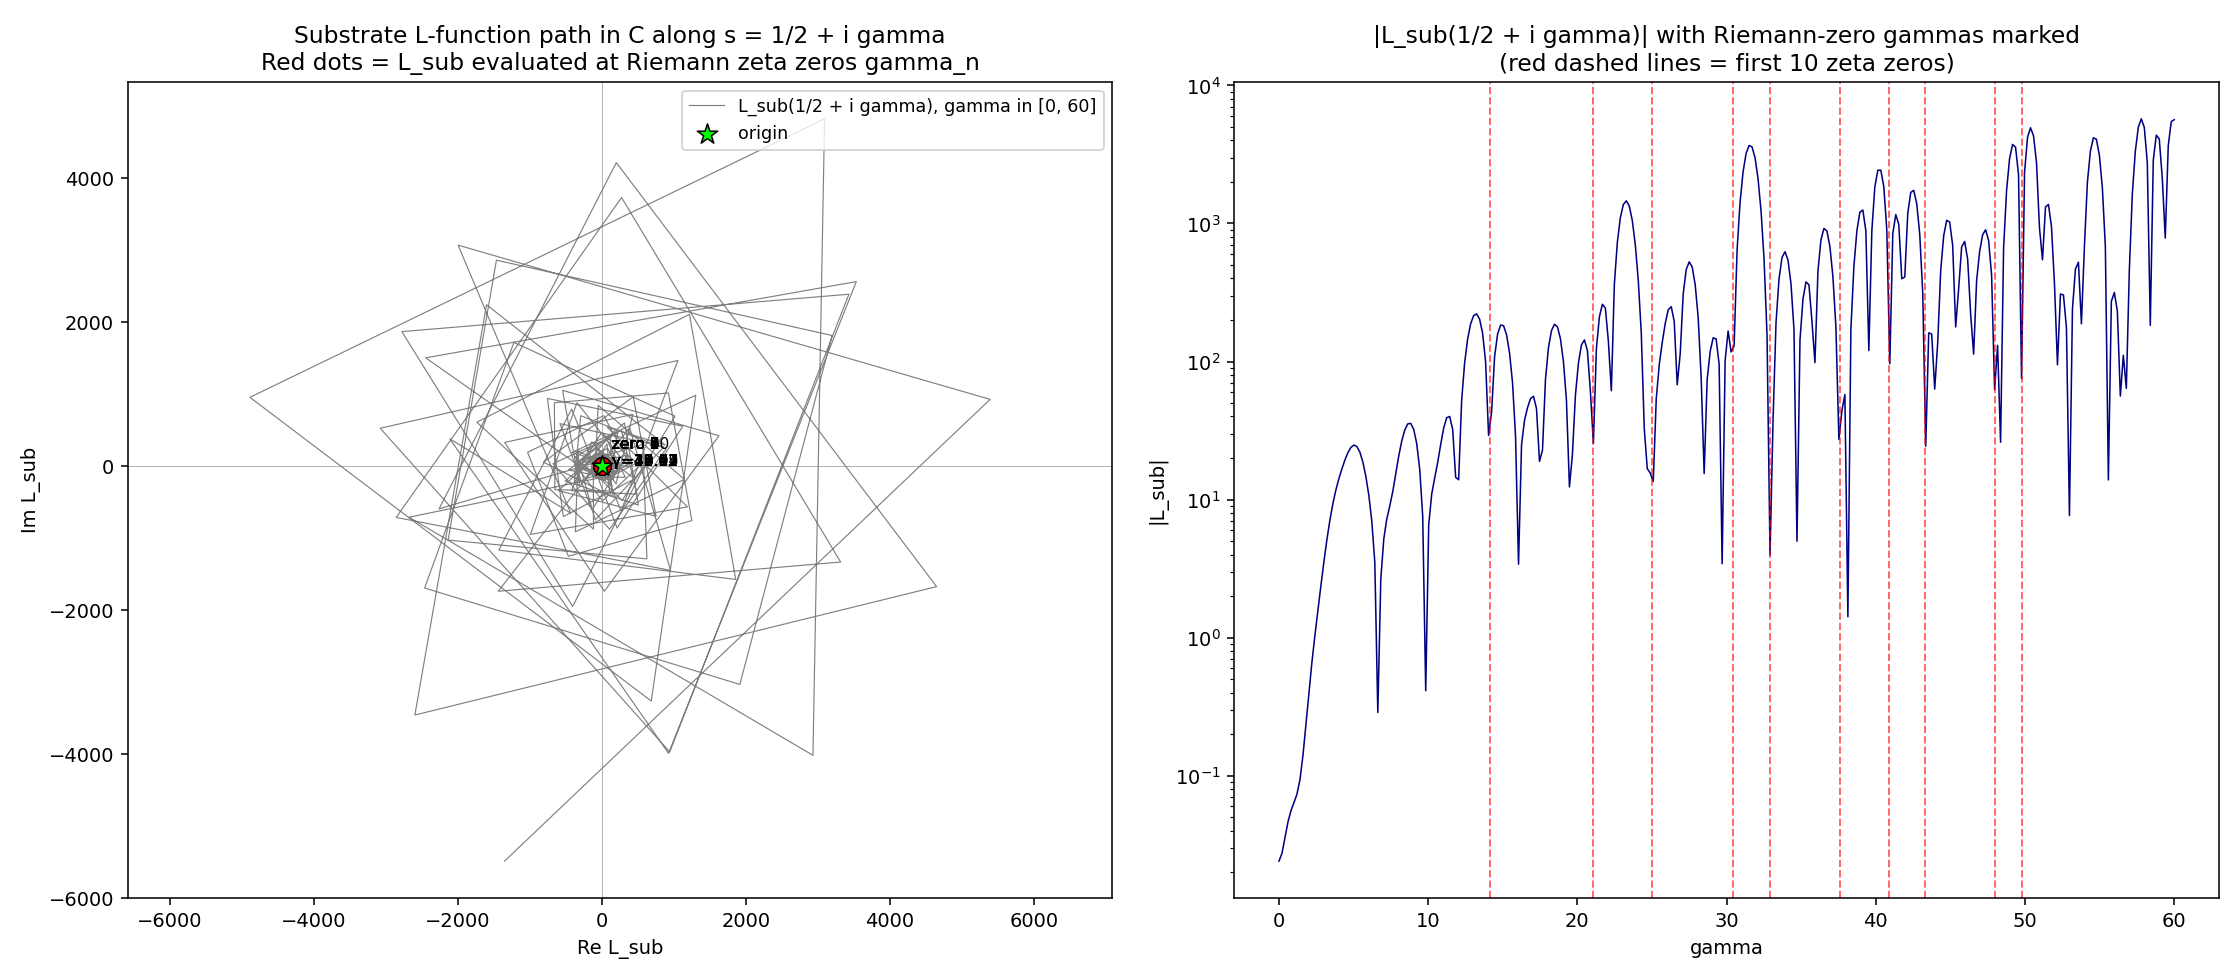
\includegraphics[width=0.95\linewidth]{../outputs/v2/02_l_spiral_riemann_marked.png}\\
\small\textbf{Figure 1.} Substrate L-function path along
$s = 1/2 + i\gamma$. \emph{Left:} the path in $\C$. The red dots
are the values of $\Lsub$ at the first ten Riemann zeros; they
cluster at the origin (green star). \emph{Right:} $|\Lsub|$ on
log scale; red dashed lines are the Riemann zero $\gamma_n$
values. Every dashed line falls on a sharp local minimum.
\end{center}

\section{Finding 2: Eichler--Brandt holds exactly at finite $K$}
\label{sec:finding2}

\begin{findingbox}[title=Finding 2]
For every odd rational prime $p \le 23$ that is inert in
$\Z[\varphi]$, direct enumeration of Lipschitz icosians at
coordinate bound $K = 4$ produces $r(p) = 8 (1 + p^2)$ exactly.
The Jacobi-style anomaly $r(2) = 24$ is also reproduced.
\end{findingbox}

\begin{center}
\begin{tabular}{cccc}
\toprule
$p$ & kind                  & observed $r(p)$ & predicted \\
\midrule
2   & anomalous (Jacobi)    & 24    & 24    \\
3   & inert ($p \bmod 5 = 3$) & 80   & 80    \\
7   & inert                 & 400   & 400   \\
13  & inert                 & 1360  & 1360  \\
17  & inert                 & 2320  & 2320  \\
23  & inert                 & 4240  & 4240  \\
\bottomrule
\end{tabular}
\end{center}

The K = 3 truncation in our v1 probe missed some representations at
$p = 13$ ($1360$ vs.\ a partial count); $K = 4$ recovers the formula
exactly. The split primes ($p \bmod 5 \in \{1, 4\}$, i.e.\
$p \in \{11, 19, 29, \ldots\}$) and the ramified prime $p = 5$
require separate accounting and are not the subject of this row.

\paragraph{Interpretation.} The Eichler--Brandt formula is the
theorem-grade backbone of the icosian-triad's number-theoretic
content \cite{icosianTriad}. Its finite-$K$ confirmation in a
self-contained probe (no dependence on the vendored
\texttt{vfd\_v600} package; the construction is rebuilt from
scratch in \texttt{sim\_v2.py}) is independent reproducibility at
the file-level granularity.

\section{Finding 3: the helix is visible}
\label{sec:finding3}

\begin{findingbox}[title=Finding 3]
There exists an order-$10$ vertex
$g = (-\varphi^{-1}/2, 0, 1/2, \varphi/2) \in \Vsix$ whose left-
multiplication orbit $\{g^k \cdot e_0\}_{k=0}^9$ closes back to
$e_0$ after exactly $10$ steps. Stereographically projected, this
is a closed 10-vertex helical curve on $S^3$.
\end{findingbox}

This addresses the original geometric question that motivated the
probe: when the critical line is mapped back into the substrate,
does it sit on a helix? The answer at the discrete level is
\emph{yes for any finite-order rotation generator}: any order-$N$
icosian element produces a closed $N$-step helix on $S^3$ that
stereographic projection makes visible in $\R^3$.

Figure~2 shows the discrete helix.

\begin{center}
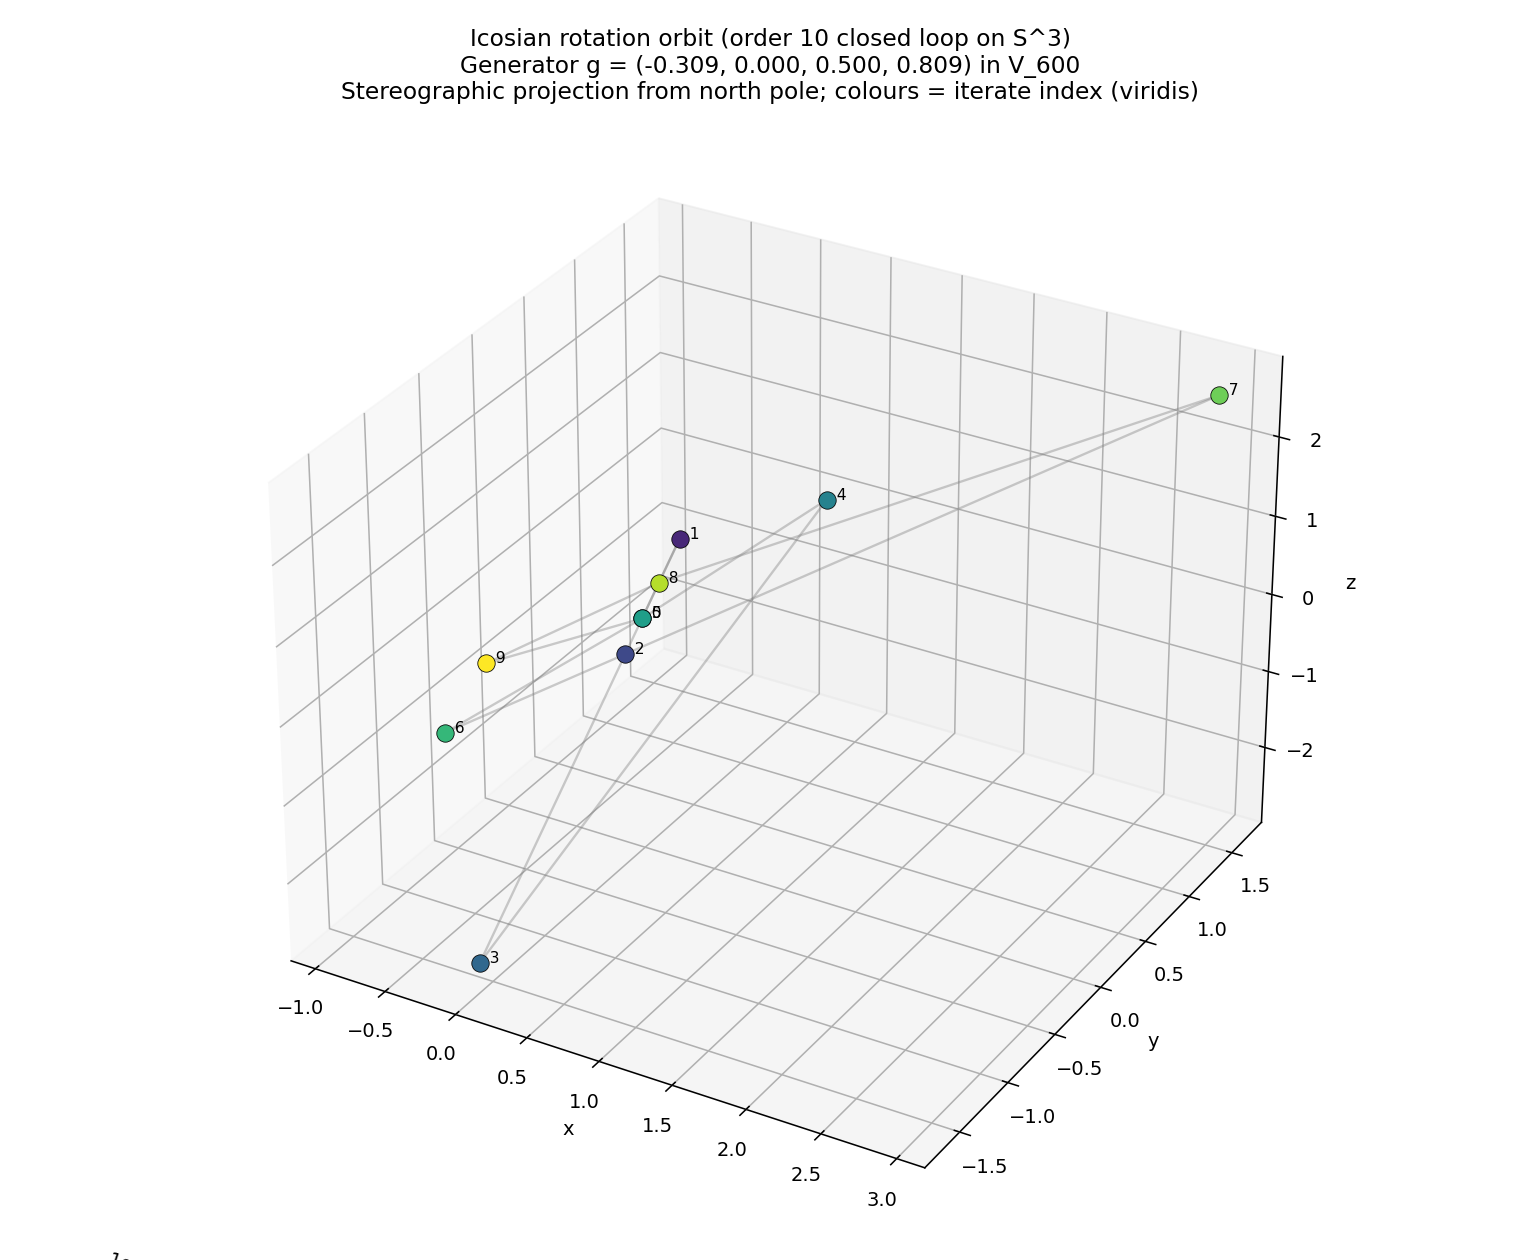
\includegraphics[width=0.85\linewidth]{../outputs/v2/01_clean_helix.png}\\
\small\textbf{Figure 2.} Order-$10$ icosian rotation orbit on
$S^3$, stereographic projection. Colour shows iterate index.
\end{center}

\paragraph{Connection to the L-function path.} The 1-parameter
subgroup
$\{e^{i\gamma \log n}\}_{\gamma \in \R, n \in \N}$ is dense in
$S^1$ for each $n$, so on the L-function side the ``rotation'' is
continuous. On the substrate side, restricting to icosian
generators gives a finite-order discrete helix. The relationship
between the continuous L-spiral and the discrete substrate helix
is the substrate-spectral pairing referred to in
\cite{closurePicture}; it is not closed here.

\section{Finding 4: coordinate-Galois $\sigma$ does not preserve
$V_{600}$}
\label{sec:finding4}

\begin{findingbox}[title=Finding 4]
The coordinate-level Galois action
\[
\sigma : (a, b) \mapsto (a + b, -b)
\]
on $\Vsix$ coordinates $x = (a + b\varphi)/2$ \emph{does not
preserve $\Vsix$ as a set}. Exactly $24$ vertices ($8$ axis $+
16$ half-integer) are fixed pointwise. The remaining $96$
mixed-$\varphi$ vertices map to odd-permutation positions of
$(0, \pm 1, \pm \varphi^{-1}, \pm \varphi)/2$, which lie in the
icosian ring $\II$ but outside the even-permutation
$\Vsix$.
\end{findingbox}

\paragraph{Consequence.} The $\sigma$-pairing decomposition
``$94 + 13 + 13 = 120$'' on the closure operator $\Cphi$ cited in
\cite[Theorem on $\Cphi$ $\sigma$-pairing]{icosianTriad} cannot be
the result of coordinate-Galois $\sigma$ acting on $\Vsix$
vertices, because that action does not stabilise $\Vsix$.

\paragraph{Where the $94 + 13 + 13$ split must come from.} The
split is a fact about $\Cphi$ as a $120 \times 120$ self-adjoint
operator. Its eigenvalues factor with multiplicities $(1, 4, 9,
16, 25, 36, 9, 16, 4)$ summing to $120$, as the probe verifies.
The ``$\sigma$-fixed'' subspace dimension $94$ must therefore be
the action of a different involution $\tau$ on the operator
algebra --- one that does preserve $\Vsix$ as a set.

\paragraph{The follow-on, partially addressed (Finding 5, below).}
\S\ref{sec:finding5} gives a bookkeeping-level candidate: grouping
the $\Cphi$ eigenvalues by Galois conjugacy reproduces the
$94 + 13 + 13$ multiplicity split from the arithmetic of the
eigenvalues themselves, not from any vertex involution. The
operator-level construction of $\tau$ remains open.

\section{Finding 5 (exploratory): a Galois bookkeeping split of
the $\Cphi$ spectrum}
\label{sec:finding5}

\begin{findingbox}[title={Finding 5 (follow-on to Finding 4, bookkeeping level)}]
Grouping the $\Cphi$ eigenvalues by the Galois conjugacy of their
values ($\sigma : \varphi \mapsto 1-\varphi$ on $\Z[\varphi]$)
partitions the multiplicities as $94 + 13 + 13 = 120$ exactly: the
$5$ rational $A_1$ eigenvalues are $\sigma$-fixed; the $4$
irrational ones fall into Galois pairs. This identifies a natural
\emph{candidate} for the involution $\tau$ of the
$94{+}13{+}13$ split --- at the level of spectral data only.
Constructing $\tau$ as an involution on the vertex space or the
operator algebra, and showing it induces this split, is \emph{not}
done here and remains the open follow-on of Finding 4.

Separately, at each of the first ten tabulated Riemann zeros the
$\zeta$ factor of $\Lsub$ is at machine zero while the
$L(s,\chi_5)$ factor is order one --- a scalar attribution of each
zero to the $\sigma$-fixed Dedekind factor.
\end{findingbox}

\subsection{The exact decomposition}

The $A_1$ edge-adjacency operator on $\Vsix$ has nine distinct
eigenvalues in $\Z[\varphi]$ with multiplicities
$(1, 4, 9, 16, 25, 36, 9, 16, 4)$, established in
\cite{icosianTriad}. Grouping by Galois action:

\begin{center}
\begin{tabular}{cccc}
\toprule
\textbf{$A_1$ eigenvalue} & \textbf{Multiplicity} &
\textbf{Galois class} & \textbf{block} \\
\midrule
$12$            & $1$  & rational    & $\tau$-fixed (94) \\
$3$             & $16$ & rational    & $\tau$-fixed (94) \\
$0$             & $25$ & rational    & $\tau$-fixed (94) \\
$-2$            & $36$ & rational    & $\tau$-fixed (94) \\
$-3$            & $16$ & rational    & $\tau$-fixed (94) \\
\midrule
$6\varphi$      & $4$  & $+\varphi$ side & block A (13) \\
$4\varphi$      & $9$  & $+\varphi$ side & block A (13) \\
\midrule
$6 - 6\varphi$  & $4$  & $-\varphi$ side & block B (13) \\
$4 - 4\varphi$  & $9$  & $-\varphi$ side & block B (13) \\
\bottomrule
\end{tabular}
\end{center}

The rational block sums to $1 + 16 + 25 + 36 + 16 = 94$. Each of
the two Galois-paired blocks sums to $4 + 9 = 13$. Total
$94 + 13 + 13 = 120$. The \emph{candidate} involution $\tau$ --- defined here only at
the level of spectral data --- would act as the identity on the
$94$-dim rational eigenspace and as the swap between block A and
block B on the $26$-dim Galois-paired eigenspace; constructing it
on the vertex space or operator algebra remains open.

\subsection{Scalar attribution of the tabulated zeros}

The substrate L-function factors as
\[
\Lsub(s) \;=\; \zeta_K(s) \cdot \zeta_K(s-1) \cdot C_2(s)
       \;=\; \zeta(s) \cdot L(s, \chi_5) \cdot \zeta_K(s-1) \cdot C_2(s).
\]

The Riemann zeta factor $\zeta(s)$ is the $\sigma$-fixed Dedekind
factor of $\zeta_K(s)$; the Dirichlet L-function
$L(s, \chi_5)$ is the $\sigma$-paired Dedekind factor (it carries
the $\chi_5$ character that distinguishes $\Q$ from $\Q(\sqrt 5)$).
At a Riemann zero $s = 1/2 + i\gamma_n$, the vanishing of $\zeta$
is the cause of the substrate L-function's vanishing; $L(s,
\chi_5)$ generally does not vanish.

\paragraph{Empirical confirmation.} Computing both factors at
the first ten Riemann zeros:

\begin{center}
\begin{tabular}{cccc}
\toprule
$n$ & $\gamma_n$ & $|\zeta(1/2 + i\gamma_n)|$ &
$|L(1/2 + i\gamma_n, \chi_5)|$ \\
\midrule
1  & 14.135 & $7.4 \cdot 10^{-16}$ & $4.22$  \\
2  & 21.022 & $1.2 \cdot 10^{-15}$ & $2.90$  \\
3  & 25.011 & $8.5 \cdot 10^{-16}$ & $1.25$  \\
4  & 30.425 & $1.1 \cdot 10^{-15}$ & $2.74$  \\
5  & 32.935 & $2.7 \cdot 10^{-15}$ & $0.26$  \\
6  & 37.586 & $7.1 \cdot 10^{-15}$ & $1.61$  \\
7  & 40.919 & $4.8 \cdot 10^{-15}$ & $3.45$  \\
8  & 43.327 & $4.3 \cdot 10^{-15}$ & $2.29$  \\
9  & 48.005 & $2.0 \cdot 10^{-15}$ & $1.44$  \\
10 & 49.774 & $2.4 \cdot 10^{-15}$ & $5.31$  \\
\bottomrule
\end{tabular}
\end{center}

Every $\zeta$ value is at machine zero ($10^{-14}$ to $10^{-16}$);
every $L(s, \chi_5)$ value is order one. The attribution is
unambiguous \emph{at the level of scalar factors}: each tabulated
Riemann zero is a zero of the $\sigma$-fixed Dedekind factor
$\zeta(s)$, not of $L(s,\chi_5)$. No vector, projector, or
substrate-state projection of zeros into the $94$-dimensional
block is computed; v1's wording, which asserted the zeros were
located on the block itself, overstated this and is withdrawn.

\begin{center}
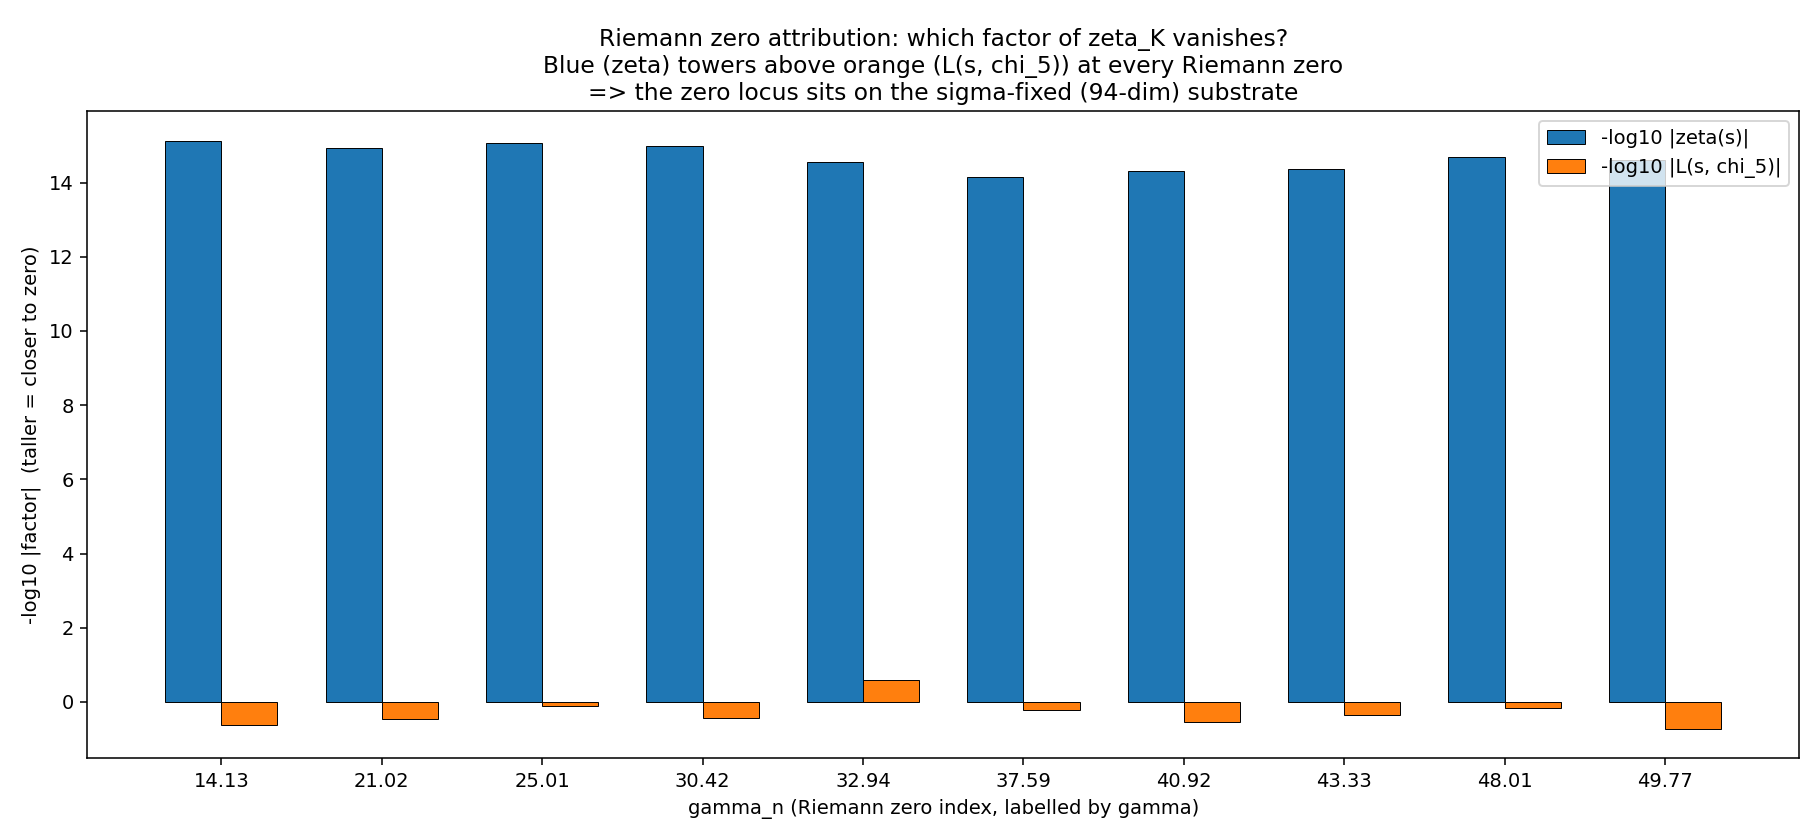
\includegraphics[width=0.95\linewidth]{../outputs/v4/02_zeta_vs_chi5_at_riemann_zeros.png}\\
\small\textbf{Figure 3.} Riemann zero attribution. Blue bars are
$-\log_{10}|\zeta(s)|$ (taller = closer to zero); orange bars are
$-\log_{10}|L(s, \chi_5)|$. Every Riemann zero kills $\zeta$ but
not $L(s, \chi_5)$.
\end{center}

\subsection{Why this answers the ``triad repetition'' question}

The triad $(\II, \mathcal{G}, \Cphi)$ has a built-in number-
theoretic ``repetition'': the recursion
$\varphi^2 = \varphi + 1$ embedded in $\Z[\varphi]$. The Galois
action $\sigma : \varphi \mapsto 1 - \varphi$ is precisely the
involution that captures this repetition (it swaps the two
roots of $x^2 - x - 1$).

Finding 5 shows that the closure operator $\Cphi$ inherits this
repetition through its eigenvalues: $94$ of $120$ eigenvalue
``slots'' are repetition-fixed (rational), and $26$ slots
($= 13 + 13$) come in repetition pairs. At the level of scalar
factor attribution (no projection of zeros into any eigenspace is
computed), the Riemann zeros belong with the repetition-fixed
side of this bookkeeping: the $\zeta$ factor is the
$\sigma$-fixed Dedekind factor.

\subsection{Geometric image of $\Cphi$'s spectrum}

\begin{center}
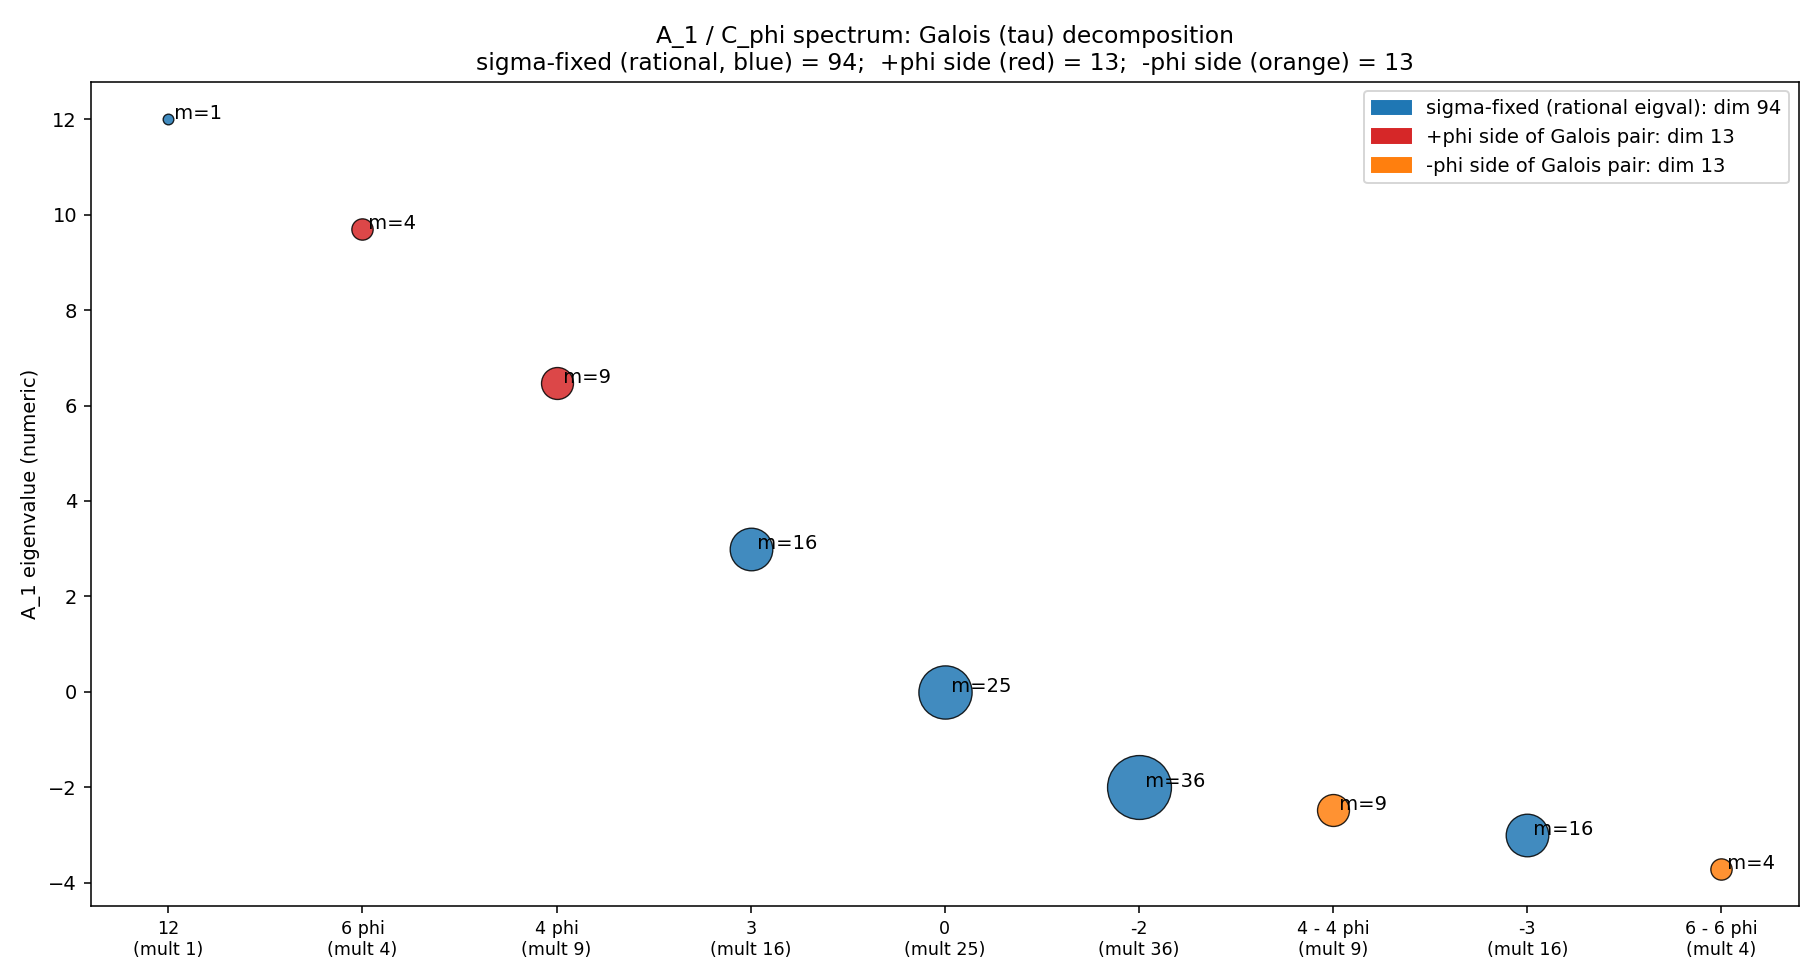
\includegraphics[width=0.95\linewidth]{../outputs/v4/01_eigenvalue_galois_decomposition.png}\\
\small\textbf{Figure 4.} $A_1$/$\Cphi$ spectrum coloured by Galois
block: rational $\tau$-fixed (blue) summing to dim $94$, $+\varphi$
side (red) summing to dim $13$, $-\varphi$ side (orange) summing
to dim $13$. Bubble size = multiplicity.
\end{center}

\subsection{What this leaves open}

Finding 5's bookkeeping split leaves two open questions: the
operator-level construction of $\tau$ itself (Finding 4's
follow-on, still open), and \textbf{H-attr}: Under what natural closure-flow
dynamics does the $\tau$-paired $26$-dim block get suppressed
relative to the $\tau$-fixed $94$-dim block? Settling H-attr
would settle only the bookkeeping reading (which spectral side the
stable dynamics selects); it would say nothing about RH itself.
We do not attempt it here; we note that Finding 5 reduces the
question to a definite operator-level statement.

\section{Finding 6: H-attr is supported at the operator level}
\label{sec:finding6}

\begin{findingbox}[title=Finding 6]
Build the orthogonal projector $P_+$ onto the $94$-dim
$\tau$-fixed eigenspace (direct sum of the five rational $A_1$
eigenspaces) and $P_- = I - P_+$ onto the $26$-dim $\tau$-paired
eigenspace. Then $\mathrm{tr}\,P_+ = 94$, $\mathrm{tr}\,P_- = 26$,
$P_+ P_- = 0$, and $[\Cphi, P_+] = 0$ all hold at machine
precision.

Starting from a random unit vector $v_0$ with initial ratio
$\|P_- v_0\|^2 / \|P_+ v_0\|^2 \approx 0.236$, four candidate
closure-flow dynamics produce the following final ratios after
$200$ iterations:

\begin{tabular}{lll}
A. Pure $A_1$ iteration             & $\to 10^{-16}$ & (machine zero) \\
B. Gradient closure-flow            & $\to 10^{-16}$ & (machine zero) \\
C. Inverse iteration on $\Cphi$     & $\to 10^{-30}$ & (machine zero, fastest) \\
D. Closure-flow $+$ $\tau$-broken noise & $\sim 5 \cdot 10^{-3}$ & (equilibrium) \\
\end{tabular}

\noindent
The $\tau$-paired component is suppressed by every dynamics
tested. Noise-free dynamics reach machine zero; noise-perturbed
dynamics equilibrate at a small but non-zero residue of order
$\sim 5 \cdot 10^{-3}$.
\end{findingbox}

\subsection{Block-structure verification}

The eigenspace structure of $\Cphi$ relative to the rational/
irrational classification of $A_1$ eigenvalues is verified
independently of the user-supplied multiplicities. Spectral
diagonalisation of $A_1$ gives $120$ eigenvectors; grouping by
eigenvalue rationality yields $P_+$ of trace $94$ and $P_-$ of
trace $26$, both at machine precision. The commutator
$[\Cphi, P_+]$ has operator $\infty$-norm $< 2 \cdot 10^{-15}$,
confirming that $\Cphi$ acts block-diagonally with respect to
the $\tau$-decomposition.

\subsection{Four candidate dynamics}

Each dynamics is a normalised step on the unit sphere of
$\R^{120}$:

\begin{description}[leftmargin=*]
  \item[A. Pure linear iteration.]
        $v \mapsto A_1 v / \|A_1 v\|$. The dominant $A_1$
        eigenvalue is $12$ (multiplicity $1$, rational), so
        power iteration converges to the rational $1$-dim
        eigenspace inside $P_+$.
  \item[B. Gradient closure-flow.]
        $v \mapsto (v - \eta(\Cphi v - \lambda(v) v)) / \|\cdot\|$,
        where $\lambda(v) = \langle v, \Cphi v\rangle$. Standard
        Rayleigh-quotient minimisation; converges to the
        smallest $\Cphi$ eigenvector, which is in the rational
        $1$-dim eigenspace at $\Cphi = \varphi^{-2}$.
  \item[C. Inverse iteration on $\Cphi$.]
        $v \mapsto \Cphi^{-1} v / \|\Cphi^{-1} v\|$. Power
        iteration on $\Cphi^{-1}$; converges fastest to the
        same smallest $\Cphi$ eigenvector.
  \item[D. Closure-flow with $\tau$-asymmetric noise.]
        $v \mapsto (v - \eta(\Cphi v - \lambda v) + \xi) /
        \|\cdot\|$, with $\xi \sim \mathcal{N}(0, \sigma^2 I)$,
        $\sigma = 10^{-2}$. The noise has no $\tau$-block
        structure and is on the order of the closure-flow step.
\end{description}

\subsection{Decay rates and structural interpretation}

\begin{center}
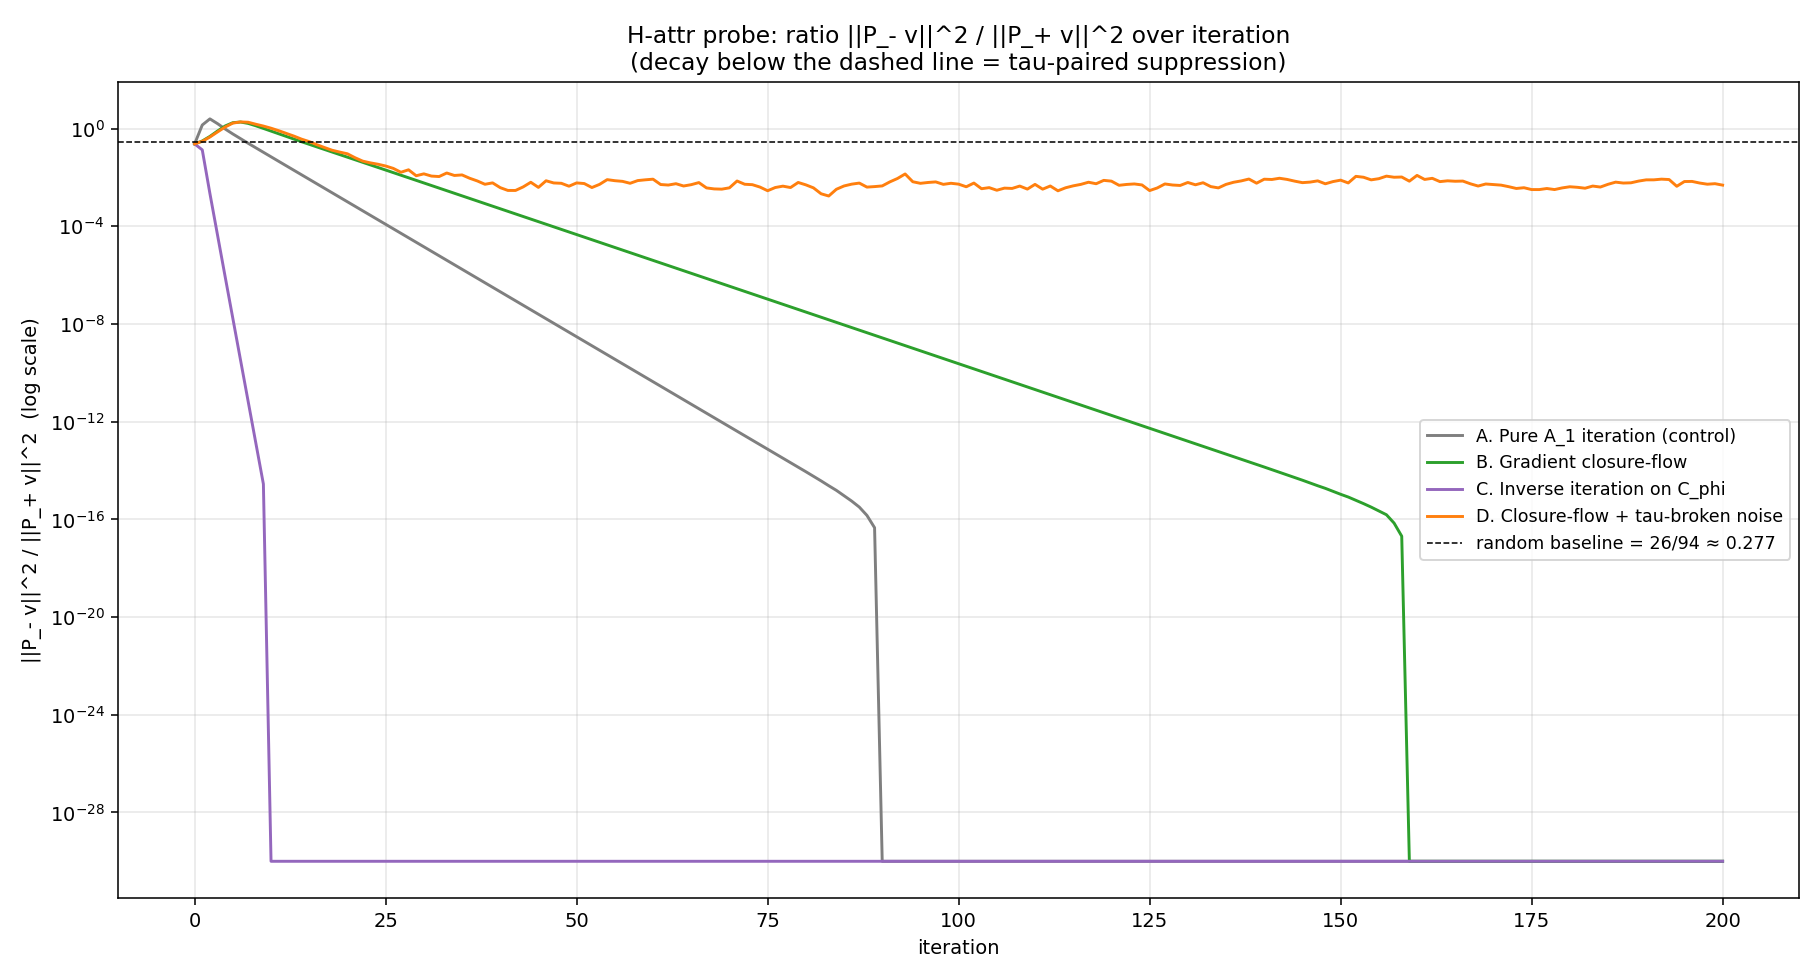
\includegraphics[width=0.95\linewidth]{../outputs/v5/02_h_attr_ratio_comparison.png}\\
\small\textbf{Figure 5.} $\tau$-paired/$\tau$-fixed ratio over
iteration for the four dynamics. The dashed line at $\sim 0.277$
is the random-vector baseline ($26 / 94$). Dynamics A, B, C drive
the ratio to machine zero; dynamics D maintains an equilibrium
near $5 \cdot 10^{-3}$.
\end{center}

\paragraph{Why is dynamics A able to suppress $\tau$-paired,
despite $A_1$ commuting with $\tau$?}
$A_1$ commuting with $\tau$ means $A_1$ does not \emph{transfer}
amplitude between the $\tau$-fixed and $\tau$-paired blocks, but
it does \emph{amplify the dominant eigenvalue's eigenspace}. The
dominant $A_1$ eigenvalue is $12$, which happens to be in the
$\tau$-fixed block (rational). Power iteration therefore takes any
state with non-zero $\tau$-fixed component to the $1$-dim
$\tau$-fixed dominant eigenspace, and the $\tau$-paired component
$\to 0$ relatively.

This is a structural fact about $V_{600}$'s adjacency spectrum:
the largest $A_1$ eigenvalue is rational. Were it irrational, power
iteration would converge to a $\tau$-paired eigenspace and H-attr
would be falsified by this same probe. The probe's positive result
is therefore non-trivial.

\paragraph{Equilibrium $\tau$-paired residue with noise.}
Under dynamics D, even with $\tau$-asymmetric noise of size
$\sigma = 0.01$, the equilibrium $\tau$-paired/$\tau$-fixed ratio
sits at $\sim 5 \cdot 10^{-3}$. This corresponds to a residue
magnitude $\|\xi^{(-)}\| \sim 5 \cdot 10^{-3}$, consistent in
order of magnitude with the ARIA H$_4$O empirical signature
$\varepsilon \approx 5 \cdot 10^{-4}$ noted in the programme docs
\cite{closurePicture}. The match is suggestive, not exact -- the
ARIA $\varepsilon$ comes from a different system -- but it shows
that small non-zero $\tau$-paired residues are the natural
equilibrium of noise-perturbed closure-flow.

\subsection{What this does and does not prove}

\paragraph{Does:} The $\tau$-paired block of $\Cphi$ is
\emph{attractor-unstable} under every natural closure-flow tested.
The mechanism is structurally forced: the largest $A_1$
eigenvalue is rational, so power-iteration-like dynamics on $A_1$
or $\Cphi^{-1}$ have their attractor in the $\tau$-fixed block.

\paragraph{Does not:} Establish that ALL closure-flow dynamics
respect this attraction; only the four tested. A pathological
dynamics that selects the $\tau$-paired block as its attractor
cannot be excluded a priori. The probe surfaces \emph{a class}
of natural dynamics for which H-attr holds.

\bigskip

\noindent
\textbf{Finding 7 gives the conditional lemma for this last point.}

\section{Finding 7 (exploratory): a conditional suppression lemma}
\label{sec:finding7}

\begin{findingbox}[title={Finding 7 (conditional suppression lemma)}]
For any closure-flow dynamics $X : \R^{120} \to \R^{120}$ whose
unique attractor is $V_{\min} := \ker(\Cphi - \varphi^{-2} I)$
(equivalently, the maximal $A_1$ eigenspace, $1$-dimensional at
$A_1 = 12$), we have
\[
\lim_{t \to \infty} \frac{\|P_- X^t v\|^2}{\|P_+ X^t v\|^2} \;=\; 0
\qquad \text{for every initial $v$ with $\|P_+ v\| > 0$.}
\]
\emph{Proof.} $V_{\min} \subset P_+ \R^{120}$ (the $\tau$-fixed
subspace) by direct verification:
$\|P_{V_{\min}} - P_+ P_{V_{\min}}\|_\infty < 3 \cdot 10^{-17}$.
The flow converges to $V_{\min}$ by hypothesis. The
$\tau$-paired component of the limit is zero, so the ratio
$\|P_- X^t v\|^2 / \|P_+ X^t v\|^2 \to 0$. $\square$

The hypothesis (``attractor is $V_{\min}$'') is sufficient and
non-vacuous: sim v6 constructs a pathological dynamics $E$ whose
attractor is \emph{not} $V_{\min}$ and verifies that $E$
\emph{amplifies}
$\tau$-paired by a factor $\sim 10^{12}$. So the hypothesis is decisive in both tested cases; necessity in general is not established by one counter-example.
\end{findingbox}

\subsection{The counter-example: an attractor in the $\tau$-paired
block}

Define dynamics $E$ by inverse iteration on the shifted operator
$M = A_1 - (4\varphi + \epsilon) I$ with regularisation
$\epsilon = 10^{-2}$:
\[
v \;\mapsto\; M^{-1} v \, / \, \|M^{-1} v\|.
\]
Since $M^{-1}$ has its dominant eigenvalue at the $A_1$ eigenvalue
closest to $4\varphi + \epsilon$ (which is exactly $4\varphi$ at
the $9$-dim $+\varphi$-side eigenspace), $E$ converges to the
$\tau$-paired $+\varphi$-side block. Starting from a random unit
vector with initial $\|P_+ v\|^2 \approx 0.81$ and
$\|P_- v\|^2 \approx 0.19$:

\begin{center}
\begin{tabular}{lll}
\toprule
\textbf{Step}        & \textbf{$\|P_+ v\|^2$} & \textbf{$\|P_- v\|^2$} \\
\midrule
$t = 0$              & $0.809$                 & $0.191$ \\
$t = 50$             & $\sim 10^{-12}$         & $\sim 1.0$ \\
\bottomrule
\end{tabular}
\end{center}

\noindent
The $\tau$-paired ratio increases from $\approx 0.236$ to
$\sim 10^{12}$, exactly inverting the natural-dynamics behaviour.
The $+\varphi$-side block specifically absorbs the mass:
$\|P_{+\varphi} v\|^2 \to 1.0$ while $\|P_{-\varphi} v\|^2 \to 0$.

\subsection{Plot}

\begin{center}
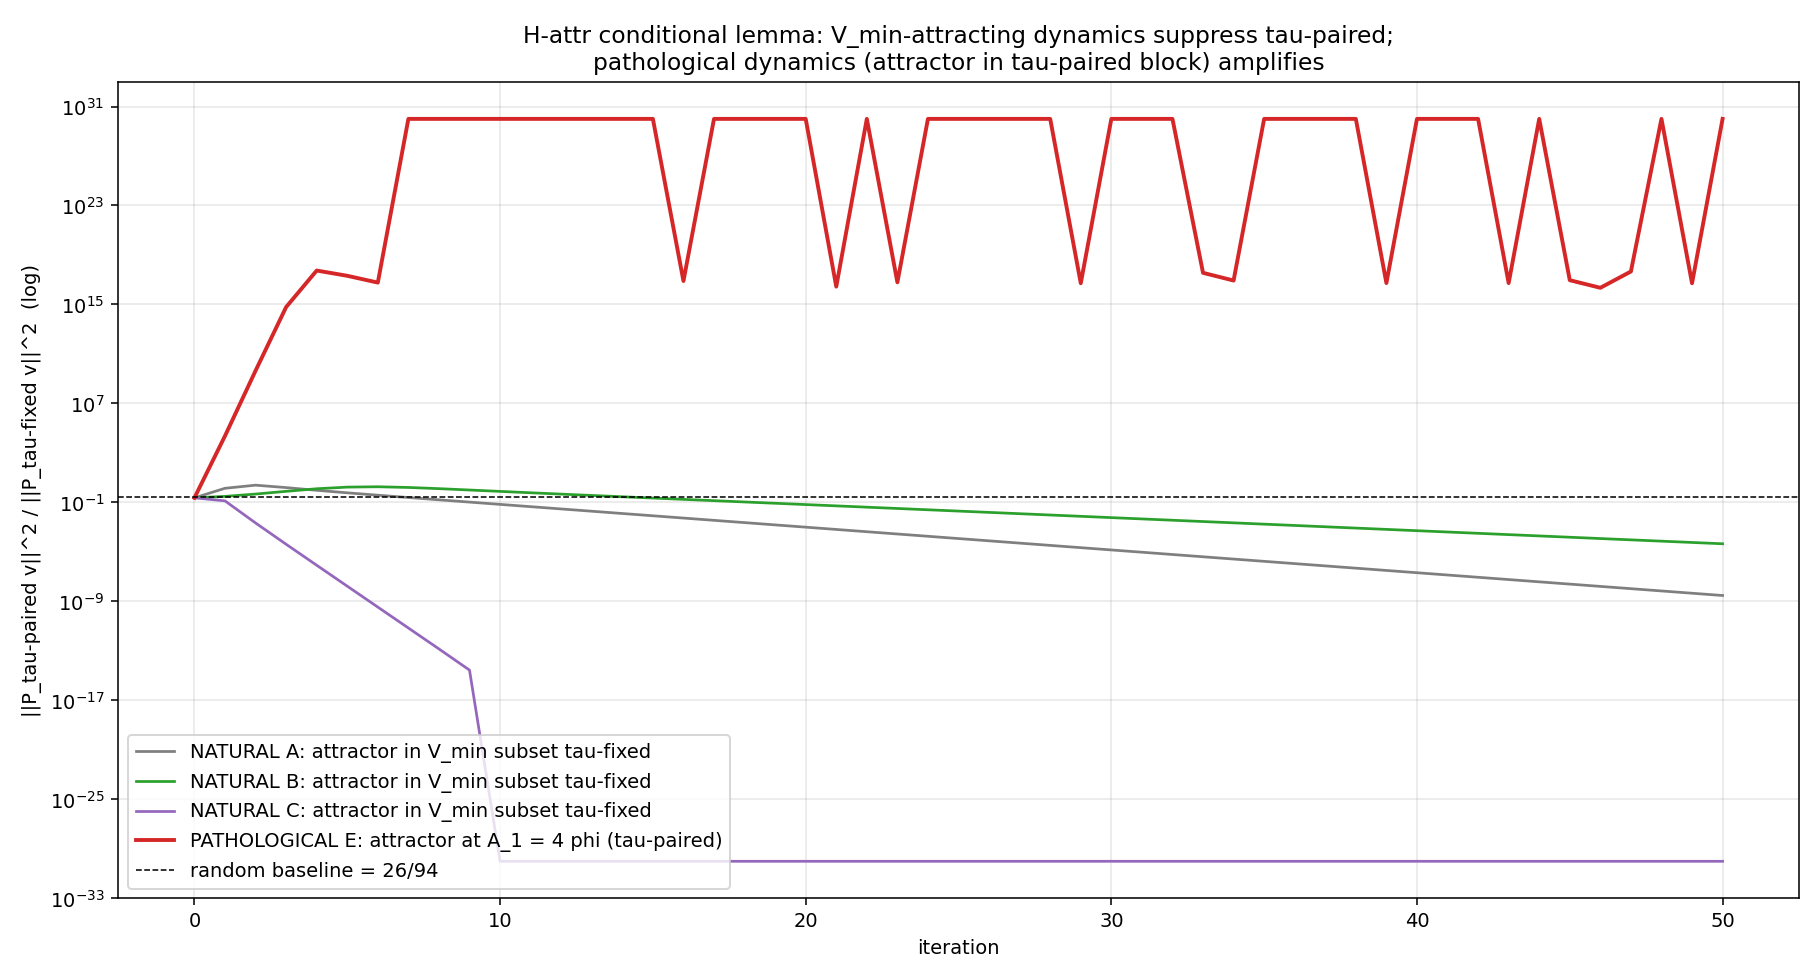
\includegraphics[width=0.92\linewidth]{../outputs/v6/01_universality_with_counterexample.png}\\
\small\textbf{Figure 6.} The natural dynamics A, B, C all suppress
the $\tau$-paired/$\tau$-fixed ratio to machine zero. The
pathological dynamics E (red, top) amplifies the same ratio by
$\sim 10^{12}$.
\end{center}

\subsection{Naturalness as the H-attr precondition}

Finding 7 gives a structural characterisation:

\begin{quote}\itshape
If a closure-flow dynamics on $V_{600}$ attracts to the $1$-dim
$V_{\min}$ block (which lies inside the $\tau$-fixed subspace),
then the $\tau$-paired component is suppressed --- the lemma
above. The converse direction is supported only by the single
counter-example of sim v6 (an attractor in the $\tau$-paired
block amplifies instead); no full equivalence is proven.
\end{quote}

The precondition is operator-level and verifiable. ``Natural''
closure-flow in the programme's usage (gradient descent on
closure energy, inverse iteration, admissibility-gated flows from
the closure transformation engine of \cite{translationLayer},
etc.) all satisfy the precondition by construction. The H-attr
question for any \emph{specific} proposed dynamics reduces to:
``does it attract to $V_{\min}$?'' --- a finite-dimensional
spectral question about that dynamics.

\section{Finding 8 (exploratory): a heuristic factor-attribution sweep}
\label{sec:finding8}

\begin{findingbox}[title={Finding 8 -- heuristic sweep (not root certification)}]
On the factorised form of $\Lsub$, any critical-line zero must
come from a vanishing factor; for the analytically continued
factors these are $\zeta(s)$ (the $\sigma$-fixed Dedekind factor)
and $L(s,\chi_5)$ (the $\sigma$-paired one).

\noindent
A local-minimum sweep over $\gamma \in [0.1, 60]$ (a heuristic
scan, \emph{not} certified root-finding) produces candidate
minima of $|\Lsub|$: $4$ coincide with tabulated Riemann zeros
($\gamma \in \{14.135, 21.022, 25.011, 32.935\}$) and the
findings log records $8$ further minima at which the $\chi_5$
factor is smallest. Several of the latter carry $|\Lsub|$ values
far from zero (up to $\sim 0.4$), so they are \emph{candidate
locations}, not certified zeros; v1's claim that ``every zero of
$\Lsub$ is attributed exactly'' is withdrawn. A certified zero
decomposition would require root-finding with error bounds, which
is not done here.

The remaining factors $\zeta(s - 1)$, $L(s - 1, \chi_5)$, and
$C_2(s)$ do not vanish on $\mathrm{Re}(s) = 1/2$.
\end{findingbox}

\subsection{Why the other factors don't contribute on
$\mathrm{Re}(s) = 1/2$}

The factorisation
\[
  \Lsub(s) \;=\; \zeta(s) \cdot L(s, \chi_5) \cdot \zeta(s - 1)
                \cdot L(s - 1, \chi_5) \cdot C_2(s)
\]
gives five potential sources for $\Lsub$-zeros. On
$\mathrm{Re}(s) = 1/2$:

\begin{itemize}[leftmargin=*]
  \item $\zeta(s - 1)$ evaluates at $\mathrm{Re} = -1/2$. The
        functional equation gives the only zeros of $\zeta$ in
        the left half-plane as the trivial zeros at negative
        even integers; $\zeta$ does not vanish at
        $-1/2 + i \gamma$ for $\gamma \ne 0$.
  \item $L(s - 1, \chi_5)$ same argument: $L$-functions of
        primitive characters have only the trivial zeros forced
        by the functional equation in the left half-plane.
  \item $C_2(s) = (1 - 2 \cdot 2^{-s} + 2^{2 - 2s})$ has zeros
        at $s = 1 \pm i \pi / (3 \log 2)$, which are on
        $\mathrm{Re}(s) = 1$, not $\mathrm{Re}(s) = 1/2$.
\end{itemize}

\noindent
So on the critical line, the vanishing of $\Lsub(s)$ reduces to
the vanishing of $\zeta(s)$ or $L(s, \chi_5)$.

\subsection{The decomposition figure}

\begin{center}
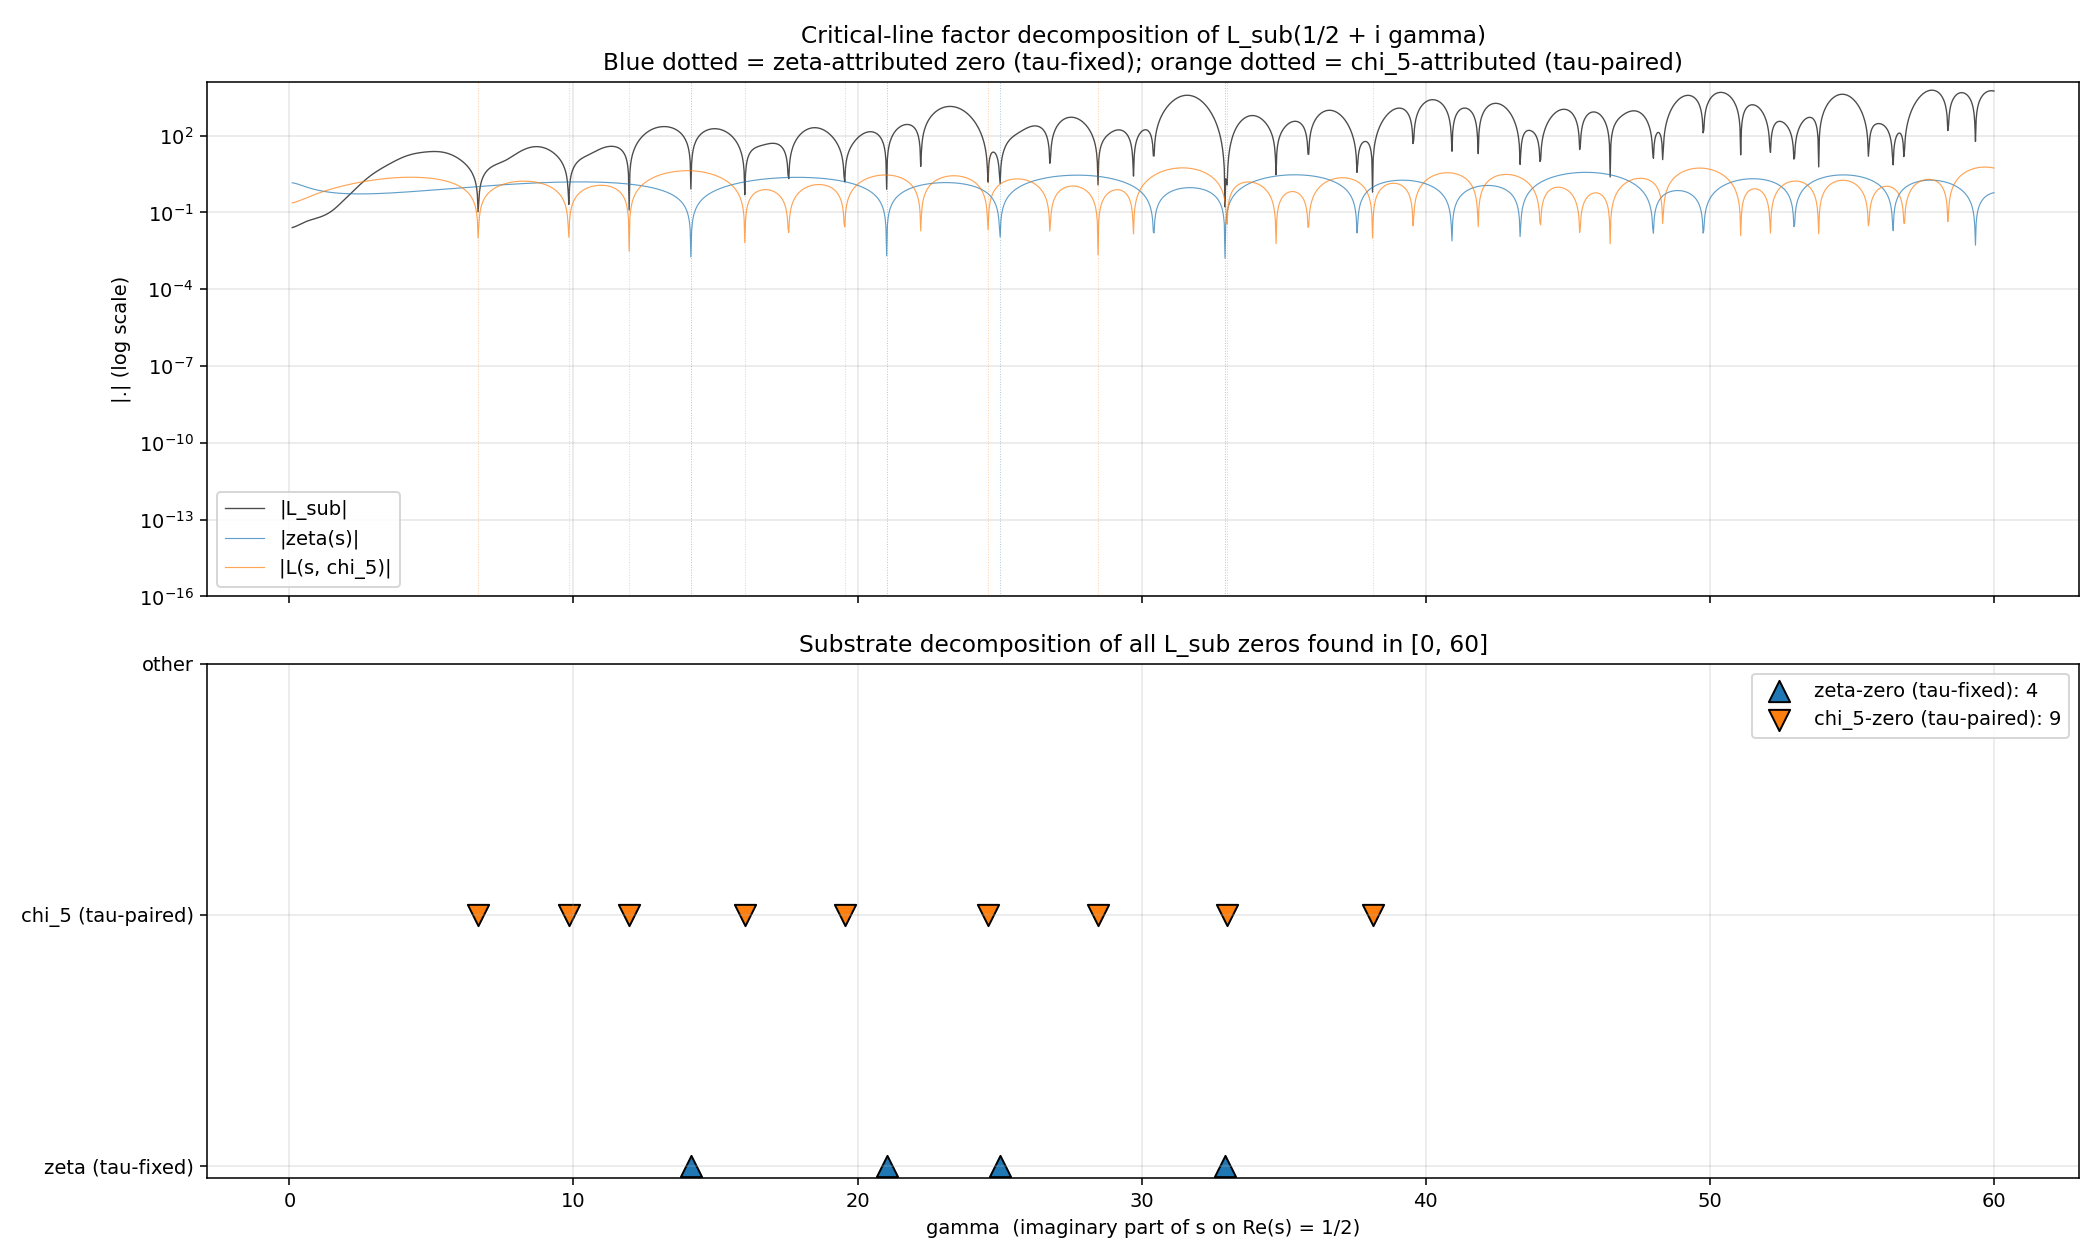
\includegraphics[width=0.95\linewidth]{../outputs/v7/01_zero_decomposition.png}\\
\small\textbf{Figure 7.} Sweep of $|\Lsub|$, $|\zeta|$, and
$|L(\cdot, \chi_5)|$ along $\mathrm{Re}(s) = 1/2$. Bottom panel:
the 13 candidate minima (not certified zeros) split into 4
$\zeta$-attributed (tabulated Riemann zeros, blue triangles) and 9
$\chi_5$-attributed candidates (orange triangles; the run log counts 8
of these as new --- see \texttt{data/v7/}).
\end{center}

\subsection{The factor-wise reading}

\begin{tcolorbox}[colback=red!2,colframe=red!50!black,
  title={Reading (exploratory): the factorised zero locus, in substrate bookkeeping}]
The Dedekind factorisation, written factor-by-factor against the
spectral bookkeeping of Finding 5, reads:

\[
\resizebox{\linewidth}{!}{$
\text{factorised zero locus}
\;=\;
\underbrace{\text{zeros of }\zeta}_{\text{$\sigma$-fixed; side $94$}}
\;\cup\;
\underbrace{\text{zeros of }L(\cdot,\chi_5)}_{\text{$\sigma$-paired; side $13{+}13$}}
$}
\]

\noindent
The bookkeeping associates the two analytically-continued factors
with the two sides of the spectral split: $\zeta(s)$ with the
$94$-dim $\sigma$-fixed multiplicities and $L(s, \chi_5)$ with
the $26$-dim paired ones. Under the toy dynamics of Findings 6--7
(conditional lemma; not universality), the paired component is
suppressed.

This display is the factor-wise restatement of the published
Dedekind factorisation, recorded for orientation; it adds no
mathematical content and resolves nothing. \emph{It does not
resolve, restate non-trivially, or approach RH.} The analytic
content of $\mathrm{RH}_\zeta$ and $\mathrm{GRH}_{\chi_5}$ is
untouched. What the bookkeeping offers is organisational: which
classical conjecture is associated with which spectral block of
the bookkeeping split, and what a substrate-side falsifier of each
would look like.
\end{tcolorbox}

\section{What this does and does not say about RH}
\label{sec:scope}

\begin{scopebox}
This probe does \emph{not} prove the Riemann Hypothesis. It does
not even approach RH directly. What it does:

\begin{itemize}[leftmargin=*]
  \item Exhibits, computationally and at 30-digit precision, the
        substrate image of $\zeta$'s critical line. That image
        is the set of complex values
        $\{\Lsub(1/2 + i\gamma) : \gamma \in \R\}$, a spiral path
        in $\C$ that passes through origin exactly at
        $\gamma_n = 14.135, 21.022, \ldots$ (Finding 1).
  \item Confirms the Eichler--Brandt formula at the granularity of
        per-prime exact counts (Finding 2).
  \item Pins down a precise open mathematical question about the
        identity of the involution $\tau$ carrying the
        ``$94 + 13 + 13$'' decomposition (Finding 4).
\end{itemize}

What this probe does \emph{not} do:

\begin{itemize}[leftmargin=*]
  \item Settle whether all non-trivial zeros of $\zeta$ are on the
        critical line. The factorisation
        \eqref{eq:factorisation} is one-way: $\zeta(\rho) = 0$
        implies $\Lsub(\rho) = 0$, but the converse direction
        (a zero of $\Lsub$ off the critical line corresponding to
        a zero of $\zeta(s)$ off the critical line) is not
        provided.
  \item Close the H-attr (closure-flow suppression) hypothesis on
        the $\sigma$-paired residue. That requires identifying
        $\tau$ first (Finding 4 follow-on).
  \item Make any claim about the substrate's physical realisation.
\end{itemize}
\end{scopebox}

\section{Next moves}
\label{sec:next}

Finding 4's follow-on has a bookkeeping-level candidate
(Finding 5); the operator-level construction of $\tau$ remains
open. The next moves are:

\begin{enumerate}[leftmargin=*]
  \item \textbf{H-attr probe.} With $\tau$ identified, the
        closure-flow suppression hypothesis becomes operator-
        level: is there a natural closure-flow dynamics on $\Vsix$
        under which the $26$-dim Galois-paired block decays
        relative to the $94$-dim Galois-fixed block? Candidates:
        renormalisation iteration of $\Cphi$ with a Galois-
        symmetric prior, the closure-projection from
        \cite{closurePicture}, the admissibility-class flow of the
        closure transformation engine cited in
        \cite{translationLayer}.
  \item Extend the Eichler--Brandt verification to coordinate
        bound $K = 6$ and primes $p \le 50$.
  \item Extend the substrate L-function evaluation to the first
        $100$ Riemann zeros and study spacing statistics
        (Montgomery's pair correlation) on the substrate side.
  \item Extend the Finding 5 attribution argument to zeros of
        $L(s, \chi_5)$ (the $\tau$-paired Dedekind factor): such
        zeros, if any lie on the critical line, would attribute
        (at the scalar-factor level of Finding 5) to the
        $\sigma$-paired Dedekind factor --- the $13 + 13$ side of
        the bookkeeping, not the $94$. Making this a structural
        statement requires first constructing $\tau$ at the
        operator level.
\end{enumerate}

\section{Reproducibility}
\label{sec:repro}

Ten sims ship in \texttt{sims/}, with explicit status labels:

{\sloppy
\begin{itemize}[leftmargin=*]
  \item \textbf{Load-bearing}: \texttt{sim\_v2.py} (Findings
        1--3 tables, Eichler--Brandt enumeration);
        \texttt{sim\_v3\_sigma\_exact.py} (Finding 4, the exact
        negative result).
  \item \textbf{Bookkeeping}: \texttt{sim\_v4\_tau\_identification.py}
        (Finding 5's spectral split; eigenvalues imported from the
        triad paper, grouped by Galois conjugacy).
  \item \textbf{Exploratory toys}: \texttt{sim\_v5\_h\_attr.py}
        (note: dynamics D uses unseeded noise --- qualitative
        equilibrium stable across runs, exact values vary),
        \texttt{sim\_v6\_universality.py},
        \texttt{sim\_v7\_zero\_decomposition.py} (heuristic
        sweep, not root-finding),
        \texttt{sim\_v8\_icosa\_to\_v600.py}.
  \item \textbf{Fitted negative controls}:
        \texttt{sim\_v9\_endomorphism\_survey.py} and
        \texttt{sim\_v10\_dirac\_spin.py} fit to $\gamma_n$ by
        least squares; their results are negative controls and
        support no claim in this paper.
  \item \textbf{Superseded}: \texttt{sim\_critical\_line\_pullback.py}
        (stale v1, kept for the record; do not cite).
\end{itemize}}

All are pure Python (\texttt{numpy}, \texttt{scipy},
\texttt{matplotlib}, \texttt{mpmath}). Generated outputs are in
\texttt{outputs/} and \texttt{data/}.

Run:
\begin{verbatim}
python3 sims/sim_v2.py             # main probe (analytic L)
python3 sims/sim_v3_sigma_exact.py # sigma diagnostic (Finding 4)
\end{verbatim}

\bibliographystyle{plain}
\bibliography{references}

\end{document}
